% ==================================================
% ChainerRL API
% Author: Lester James V. Miranda
% ==================================================

\documentclass[preview, convert={outfile=\jobname-out.png,density=300}]{standalone}

\usepackage{tikz}
\usepackage{color}
\usepackage{subfig}
\usepackage{ifthen}
\usepackage{graphicx}

\renewcommand\familydefault{\sfdefault}

\usetikzlibrary{
    matrix,
    shapes,
    fit,
    arrows,
    positioning,
    calc,
    backgrounds,
    shadows.blur,
    shapes.geometric,
}

\begin{document}
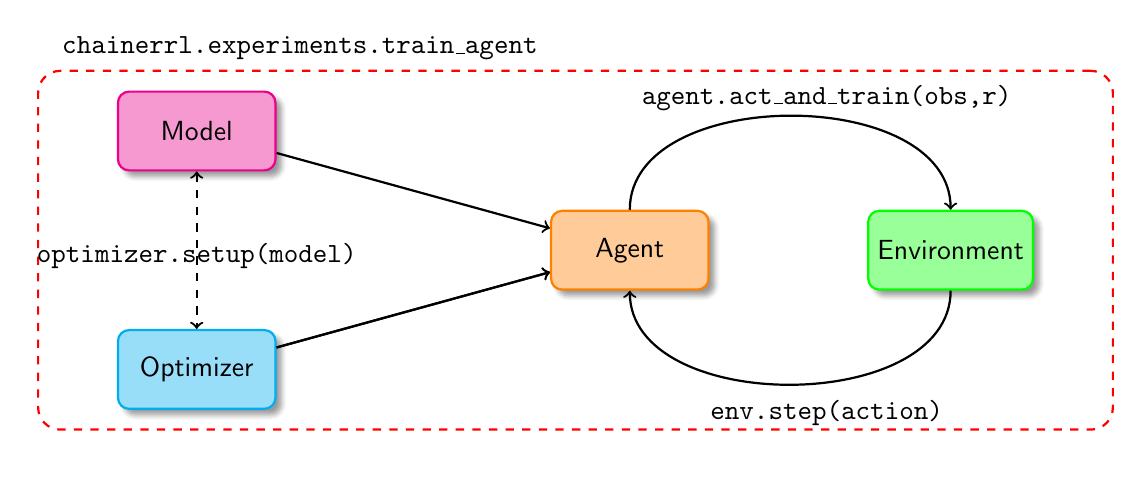
\begin{tikzpicture}[
    node distance= 2cm,
    module/.style={draw, thick, rounded corners, text=black, align=center,
                minimum width=2cm,minimum height=1cm,fill=white, 
                blur shadow={shadow blur steps=5}},
    model/.style={module, fill=magenta!40, draw=magenta, text=black},
    optimizer/.style={module, fill=cyan!40, draw=cyan, text=black},
    agent/.style={module, fill=orange!40, draw=orange, text=black},
    environment/.style={module, fill=green!40, draw=green, text=black},
    episode/.style={draw, color=red, fill=none, rounded corners=8pt,thick, inner xsep=1cm, inner ysep=0.25cm},
]

\node[model] at (0,0) (model) {Model};
\node[optimizer] (optimizer) [below= of model] {Optimizer};
\node[agent] at ([xshift=5.5cm]$(model)!0.5!(optimizer)$) (agent) {Agent};
\node[environment] (env) [right= of agent] {Environment};

\draw[<->, thick, dashed] (model) -- (optimizer) node[yshift=-0.5cm,midway, label={\texttt{optimizer.setup(model)}}] (setup) {};
\draw[->, thick] (model) -- (agent) {};
\draw[->, thick] (optimizer) -- (agent) {};
\draw[->, thick] (optimizer) -- (agent) {};
\draw[->, thick] (agent) to[out=90, in=90] (env) node[midway, xshift=8cm, label={\texttt{agent.act\_and\_train(obs,r)}}] (batchAct) {};
\draw[->, thick] (env) to[out=-90, in=-90] (agent) node[midway, yshift=-4cm, xshift=8cm, label={\texttt{env.step(action)}}] (step) {};

\begin{scope}[on background layer]
    \node [episode, dashed, fit=(model)(optimizer)(env)(setup)(batchAct), label={[xshift=-3.5cm]\texttt{chainerrl.experiments.train\_agent}}] {};
\end{scope}

\end{tikzpicture}
\end{document}

